\subsection{Bachelor in Physik}
\label{subsec:studienstruktur_bsc_physik}
% Problem mit \bigskip: manche Wörter des Satzes nach \bigskip werden anscheinend nicht mitgenommen. Kann man mit \FloatBarrier lösen. Aber zweimal \\ scheint auch zu funktionieren und ist "built-in."
Glücklicherweise seid ihr nicht mehr die ersten, die in Frankfurt auf Bachelor studieren. Ab dem letzten Semester gibt es einen neuen, überarbeiteten Studiengang Physik. Ihr könnt also von den Erfahrungen der vergangenen Semester profitieren. Der alte Studiengang BSc. Physik wurde nämlich im Wesentlichen beibehalten und an einigen Stellen verbessert.\\
Innerhalb der sechs Semester bis zum Bachelor müsst ihr viele Veranstaltungen besuchen; was in welchem Semester dran kommt, soll euch die folgende Aufstellung zeigen. Akut wichtig ist natürlich erstmal euer
% Alternative zu subsubsection:
\\\\\hspace*{\fill}\textbf{Erstes Semester}\hspace*{\fill}\\\\
%\subsubsection*{Erstes Semester}
%\label{subsubsec:studienstruktur_bsc_physik_semester1}
In eurem ersten Semester sollt ihr mindestens drei Vorlesungen besuchen:\\
In der \fach{Experimentalphysik} kommt die Vorlesung \VL{Experimentalphysik 2: Elektrodynamik}, die das Modul \Modul{VEX2} bildet, auf euch zu. Die Vorlesung werdet ihr gemeinsam mit den Studierenden hören, die ihr Studium im letzten Wintersemester begonnen haben. Dies stellt aber kein Problem dar, da diese Vorlesung keine besonderen Vorkenntnisse benötigt werden. Dieses Modul bringt 8 CP's und ihr müsst dafür eine Klausur schreiben.\\
Ob es für euch sinnvoll ist, jetzt schon ein \fach{Nebenfach} zu belegen,
hängt davon ab, welches ihr nehmen wollt. Seht hierzu den Abschnitt ab Seite \pageref{sec:nebenfach} über Nebenfächer.\\
Um euer Studium zügig voranzutreiben, ist es sinnvoll, eines der Anfängerpraktika in den ersten beiden Semestern abzuschlie\ss en. Wir empfehlen euch, mit dem \VL{AP 2} zu beginnen, da ihr zuerst die Vorlesung \VL{Elektrodynamik} hört und das \VL{AP 2} auf diese Themen ausgerichtet ist. Ihr könnt es entweder jetzt schon machen oder als Blockpraktikum in der vorlesungsfreien Zeit vor dem Wintersemester oder auch im Wintersemester. Da die Plätze in den Praktika aber nicht ausreichen, ist es sehr üblich und auch normal, dass die Hälfte eines Jahrgangs zuerst in das \VL{AP 1} geht. Die Praktika, die ihr im ersten bis dritten Semester hinter euch bringen solltet, bilden die Module \Modul{PEX1} und \Modul{PEX2}. Die Studienleistungen hierzu sind eure Protokolle, die Module sind \textbf{unbenotet}.
Wieviele Versuche und Protokolle von euch verlangt werden, hängt von der Länge des Semesters ab.
Praktika werden in Zweier--Gruppen bestritten.
%\pagebreak
\\\\\hspace*{\fill}\textbf{Zweites Semester}\hspace*{\fill}\\\\
%\subsubsection*{Zweites Semester}
%\label{subsubsec:studienstruktur_bsc_physik_semester2}
In der \fach{Experimentellen Physik} besucht ihr nun die Vorlesungen \Modul{VEX1A} \VL{Mechanik} und \Modul{VEX1B} \VL{Thermodynamik}. Diese zwei Veranstaltungen sind so auf das Semester verteilt, dass ihr bis zu den Weihnachtsferien im Dezember die Vorlesung Mechanik besucht und ab Januar die Vorlesung Thermodynamik. Es handelt sich dabei um zwei einzelne Module; über Mechanik schreibt ihr keine Klausur, dafür am Ende des Semesters über Thermodynamik.\\
Eure theoretische Physikvorlesung behandelt in diesem Semester die \VL{Mathematische Methoden der Theoretischen Physik}. Es gibt 8 CP's für das Modul \Modul{VTH1}.\\
Im zweiten Semester beginnt ihr mit eurem dritten Haptfach \fach{Mathematik}. Ihr werdet zusammen mit den Wintersemester--Anfängern die Vorlesung \VL{Mathematik für Studierende der Physik 1} aus dem Modul \Modul{VMATH1} hören, die 8 CP's bringt und mit einer Klausur abgeschlossen wird.\\
Im Wintersemester kann man die meisten Nebenfächer beginnen. Wenn ihr im ersten Semester noch kein \fach{Nebenfach} gewählt habt, ist nun der richtige Zeitpunkt, eins zu belegen.
%\subsubsection*{Drittes Semester}
%\label{subsubsec:studienstruktur_bsc_physik_semester3}
\\\\\hspace*{\fill}\textbf{Drittes Semester}\hspace*{\fill}\\\\
In der Experimentalphysik sind in diesem Semester zwei Vorlesungen vorgesehen, die die Module \Modul{VEX4A} und \Modul{VEX4B} bilden. Die Vorlesungen behandeln \VL{Kernphysik} und \VL{Festkörperphysik}, bringen jeweils 4 CP und werden am Ende des Semesters einzeln abgeprüft.\\
In \fach{Theo} ist es die \VL{Mechanik}, die ihr besuchen müsst.
Es handelt sich wieder um eine Vorlesung über 8 CP, die am Ende des Semesters durch eine Klausur abgeprüft wird.\\
In der Mathematik hört ihr die Vorlesung \VL{Mathematik für Studierende der Physik 2} aus dem Modul \Modul{VMATH2}, die ebenfalls 8 CP's bringt und mit einer Klausur abgeschlossen wird.\\
Im dritten Semester absolviert ihr nun euer zweites Anfängerpraktikum, entsprechend der Wahl im 2. Semester also das \VL{AP 1} oder \VL{AP 2}.
Jedes der \fach{Praktika} bringt euch 8 unbenotete CP's.
\begin{figure}[p]
  	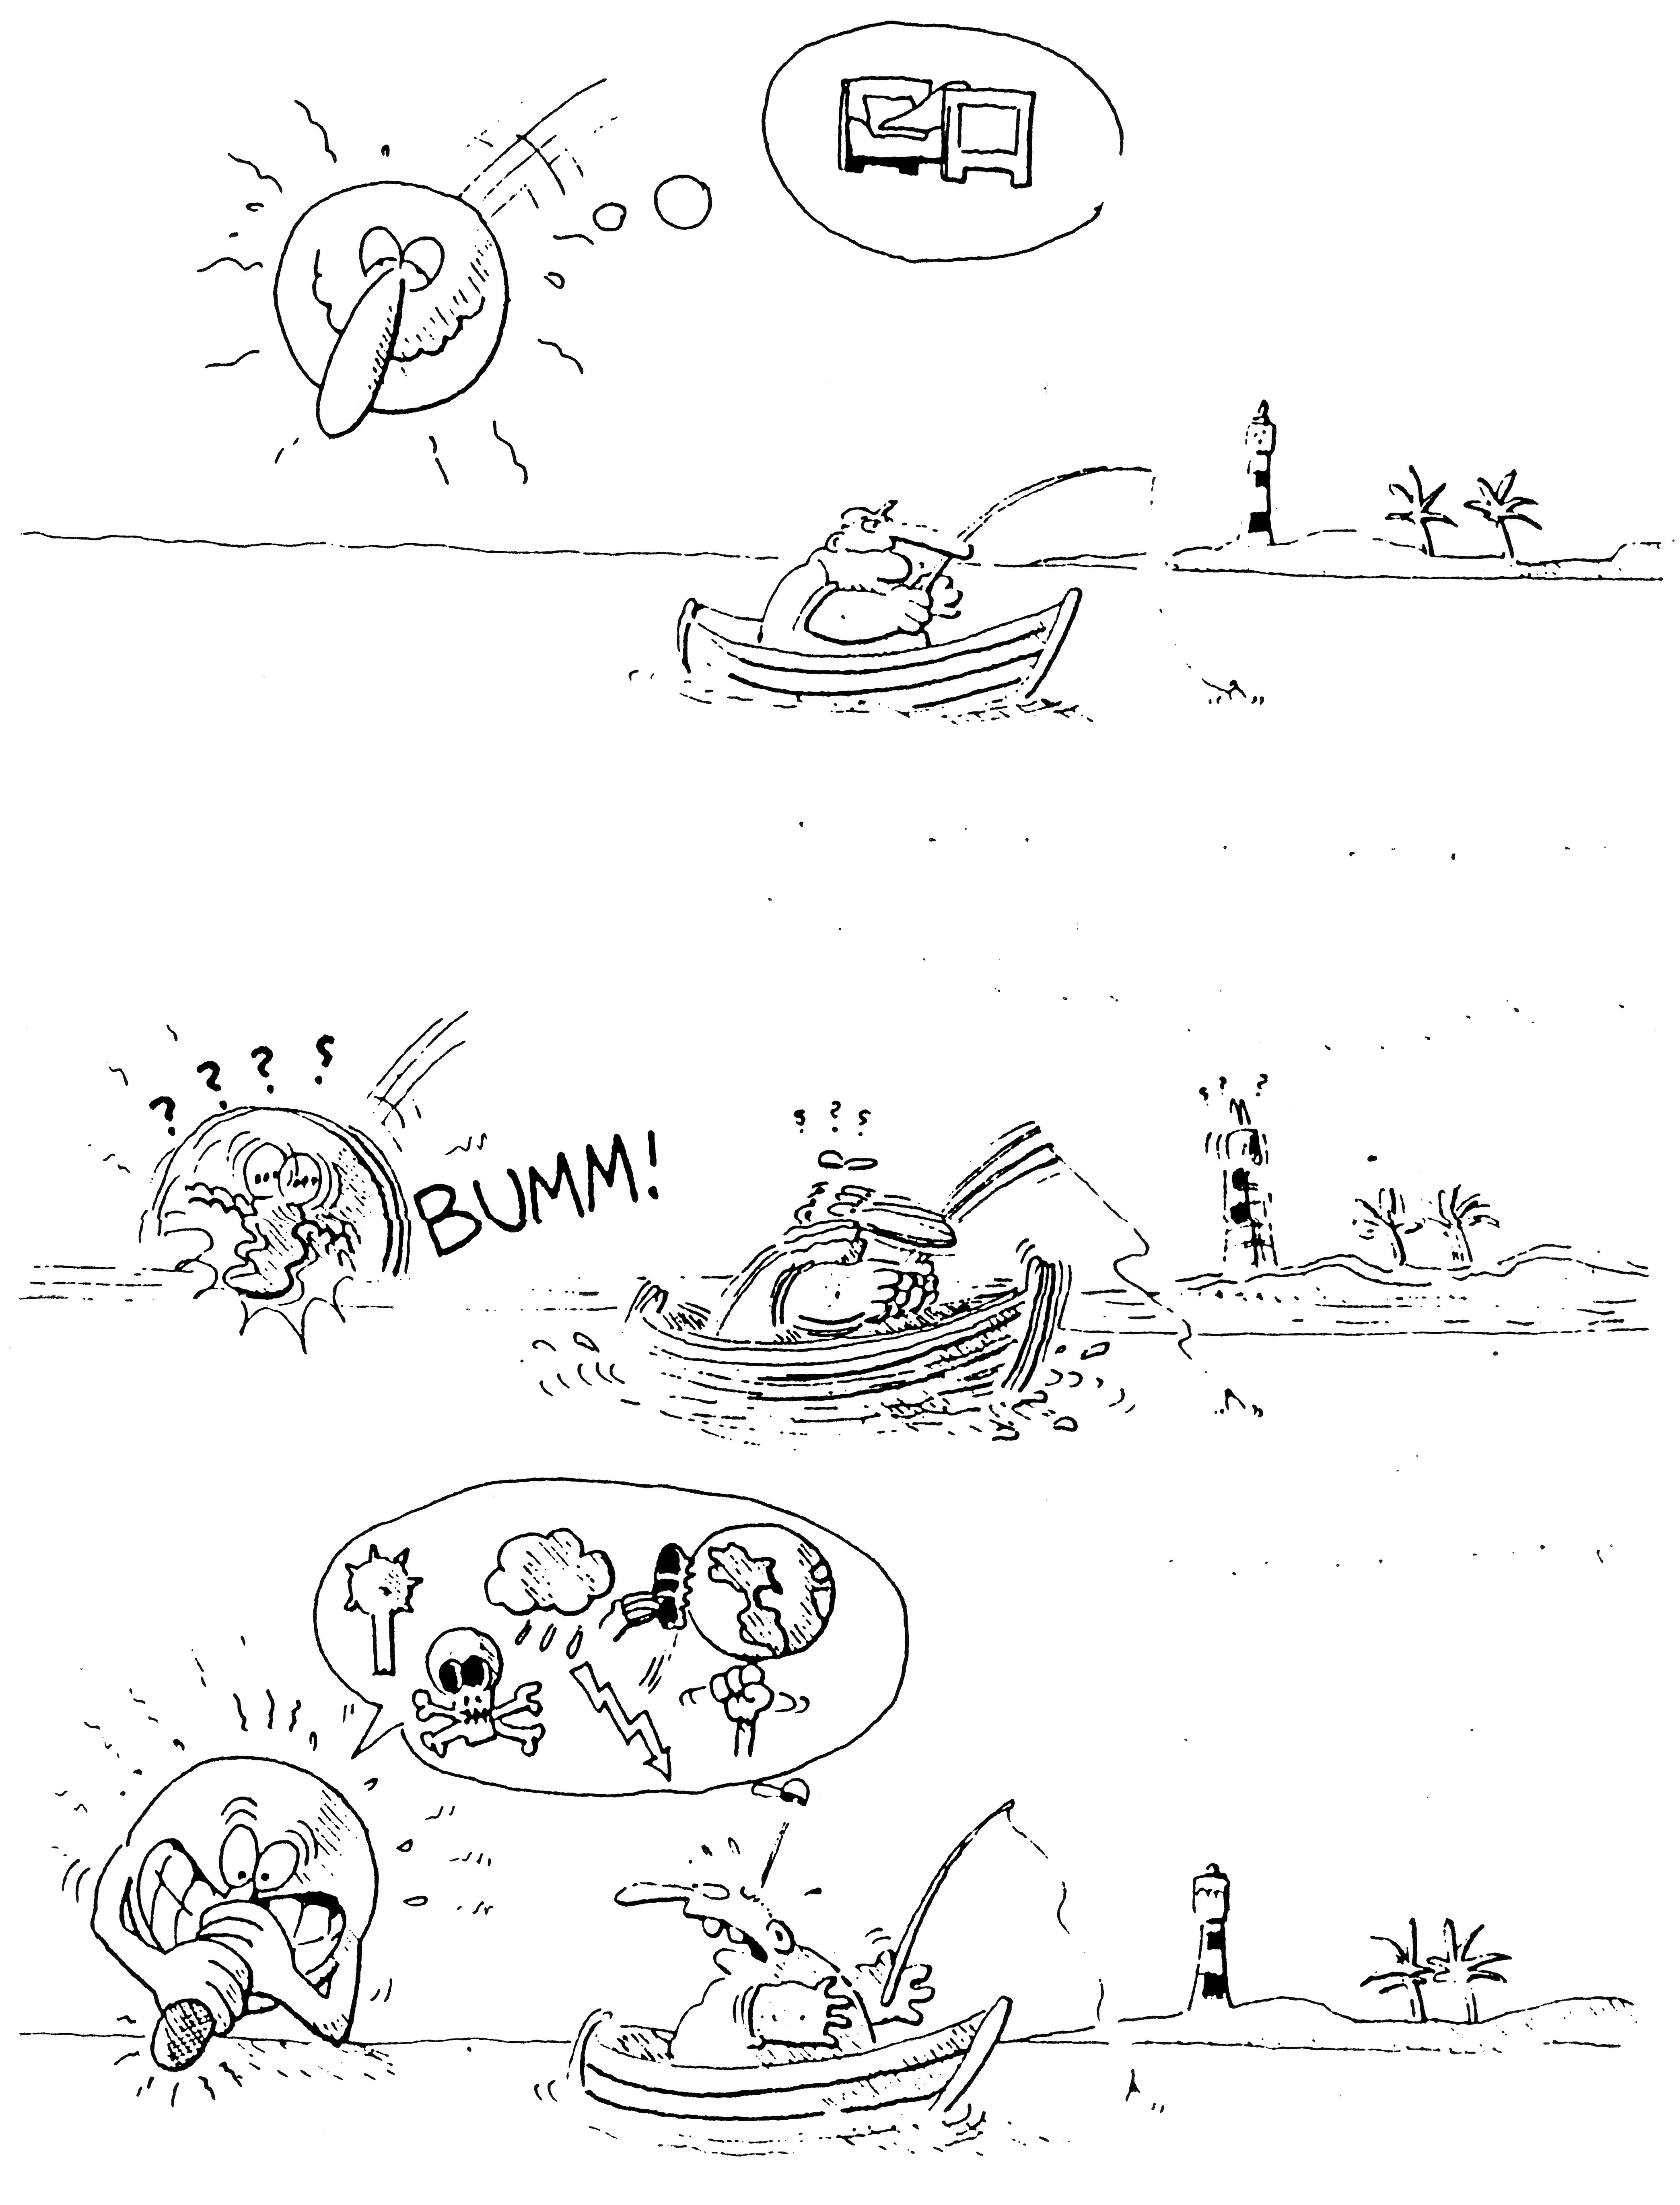
\includegraphics[height=\textheight]{\imgdir/sonnendotz.jpg}
\end{figure}
%\subsubsection*{Viertes Semester}
%\label{subsubsec:studienstruktur_bsc_physik_semester4}
\\\\\hspace*{\fill}\textbf{Viertes Semester}\hspace*{\fill}\\\\
Im vierten Semester steht wieder ein \fach{Praktikum} auf dem Programm, das \VL{Pro\-grammier\-praktikum}, in dem ihr für Physiker wichtige Programmierkenntnisse erlernt (Modul \Modul{PPROG}, 4 CP). Auch dieses Praktikum ist unbenotet.\\
Für dieses Semester sind in der Experimentalphysik zwei Vorlesungen vorgesehen, die zusammen das \Modul{VEX3} bilden. Die Vorlesungen behandeln \VL{Optik} und \VL{Atomphysik}, bringen jeweils 4 CP und werden am Ende des Semesters in einer gemeinsamen Modulabschlussklausur geprüft.\\
Eure Mathematikausbildung schlie\ss t ihr nun mit der Vorlesung \VL{Mathematik für Studierende der Physik 3} ab. Das Modul \Modul{VMATH3} bringt nach Bestehen einer Klausur auch 8 CP's.\\
Auch in der \fach{Theoretischen Physik} steht in diesem Semester die \VL{Elektrodynamik} an, die wiederum 8 CP's zählt und mit einer Klausur abgeprüft wird.\\
Langsam solltet ihr mit den \Modul{Wahlpflichtveranstaltungen}\label{Wahlpflicht} anfangen. Hier könnt ihr aus einer Vielzahl von Veranstaltungen wählen (manche sind aber erst ab dem fünften Semester geeignet), ihr müsst insgesamt zwischen 10 und 16 Credit Points (das sind etwa 3-5 Vorlesungen) nachweisen. Jede Veranstaltung wird, wenn überhaupt, einzeln geprüft. Wahlpflicht- und Nebenfachbereich zusammen ergeben ungefähr 19~\% der Bachelor-Endnote.\\
Die Wahlpflichtveranstaltungen sollen euch Gelegenheit bieten, euch in den einzelnen Arbeits- und Forschungsbereichen umzuschauen und die Auswahl für euer Arbeitsgebiet in der Bachelor-Arbeit einzugrenzen oder zu treffen.
%\subsubsection{Fünftes Semester}
%\label{subsubsec:studienstruktur_bsc_physik_semester5}
\\\\\hspace*{\fill}\textbf{Fünftes Semester}\hspace*{\fill}\\\\
Langsam wird es ernst, euer letztes Praktikum läuft. Es ist das \VL{Fortgeschrittenen-Praktikum}, in dem ihr ähnlich wie im Anfängerpraktikum Versuche durchführen und Protokolle abgeben müsst (Modul \Modul{PEXF}, 12 CP).\\
In der \fach{Theoretischen Physik} wird in diesem Semester die \VL{Quantenmechanik} behandelt, die wiederum 8 CP's zählt und mit einer Klausur abgeprüft wird.\\
Au\ss erdem habt ihr in diesem Semester viel Zeit für Wahlpflicht und Nebenfach.
%\subsubsection{Sechstes Semester}
%\label{subsubsec:studienstruktur_bsc_physik_semester6}
\\\\\hspace*{\fill}\textbf{Sechstes Semester}\hspace*{\fill}\\\\
Das sechste Semester sollte für die Bachelor-Arbeit zur Verfügung stehen. Jedoch werdet ihr auch noch in der \fach{Theoretischen Physik} die  \VL{Thermodynamik und Statische Physik} behandeln, die wiederum 8 CP's zählt und mit einer Klausur abgeprüft wird.\\
Hier sollt ihr noch ein Seminar besuchen - das im Regelfall das Arbeitsgruppen-Seminar sein wird, in der ihr die Bachelor-Arbeit macht. Einige Wahlpflichtveranstaltungen sind noch für das sechste Semester vorgesehen.\\
Das Seminar ist nicht benotet, und die Bachelor-Arbeit ergibt 11,8~\% der Gesamtnote.
\\\\\textbf{Anmerkung}\hspace*{\fill}\\\\
%\paragraph{Anmerkung:}
Zur Feststellung der Noten wird folgendes System verwendet:\\
In der Experimentalphysik schreibt ihr fünf Klausuren
(\VL{Thermodynamik}, \VL{Elektrodynamik}, \VL{Atomphysik und Optik}, \VL{Kernphysik}, \VL{Festkörperphysik}), die ihr alle bestehen müsst.
In die Endnote gehen aber nicht alle Klausurnoten ein. Es werden Noten im Gesamtgewicht von mindestens 20 CP gewertet. Man kann also Noten im Umfang von 8 CP aus der Wertung auslassen. Diese Experimentalphysik-Note zählt 25,2~\% der Gesamtnote.\\
In der theoretischen Physik ist das System ähnlich, aber ein wenig einfacher: Ihr schreibt vier Klausuren, die alle mit 8 CP's das gleiche Gewicht haben. Die besten drei dieser vier Noten werden ausgewählt, gemittelt und zählen wie in Ex 25,2~\% der Gesamtnote.\\
In der Mathematik ist es fast genau so: Ihr schreibt drei Klausuren mit dem selben Gewicht; hiervon gehen die besten beiden gemittelt zu 18,9~\% in die Gesamtnote ein.
%\subsubsection{Tabellarische Semesterübersicht}
\\\\\hspace*{\fill}\textbf{Tabellarische Semesterübersicht}\hspace*{\fill}\\\\
\noindent
\begin{tabular}{|p{.13\textwidth}||p{.17\textwidth}|p{.17\textwidth}|p{.17\textwidth}|p{.19\textwidth}|}
	\hline
	\textbf{Phy 1} & Ex & \multicolumn{2}{c|}{Nebenfach} & Praktika \\
	\hline \hline
  	Vorlesung & \VL{Elektro\-dynamik} & \VL{Nebenfach 10-16 CP} & \VL{siehe Abschnitt Nebenfach} & \VL{Anfänger\-praktikum~II} \\
	Aus Modul & \Modul{VEX2} & \multicolumn{2}{c|}{\Modul{VTHS}} & \Modul{PEX2} \\
 	Stunden & 4+2 & & & 4 \\
 	CP & 8 & & & 8 \\
  	Benotet? & \textsl{benotet} & textsl{benotet} &  & \textsl{unbenotet} \\
  	\hline
\end{tabular}
\\
\noindent
\begin{tabular}{|p{.13\textwidth}||p{.17\textwidth}|p{.17\textwidth}|p{.17\textwidth}|p{.19\textwidth}|}
	\hline
  	\textbf{Phy 2} & Ex & Theo & Mathe & Sonstiges \\
  	\hline \hline
  	Vorlesung & \small{\VL{Mechanik}, ab Weihnachtspause \VL{Thermodynamik}} & \VL{Mathematische Methoden der Theoretischen Physik} & \VL{Mathe I} & Nebenfach \\
  	Aus Modul & \Modul{VEX1A}, \Modul{VEX1B} & \Modul{VTH1} & \Modul{VMATH1} & \\
  	Stunden & 5+2, 5+2 & 4+2 & 4+2 & insges. \\
  	CP & 6, 4 & 8 & 8 & 16-22 CP \\
  	Benotet? & \textsl{unbenotet}, \textsl{benotet} & \textsl{benotet} & \textsl{benotet} & \textsl{benotet} \\
  	\hline
\end{tabular}
\\
\noindent
\begin{tabular}{|p{.13\textwidth}||p{.17\textwidth}|p{.17\textwidth}|p{.17\textwidth}|p{.19\textwidth}|}
	\hline
  	\textbf{Phy 3} & Ex & Theo & Mathe & Praktika \\
  	\hline \hline
  	Vorlesung & \small{\VL{Kerne~\&~Teil\-chen}, \vfill \VL{Festkörper}} & \VL{Quanten\-mechanik} & \VL{Mathe II} & \VL{Anfänger-Praktikum~I} \\
  	Aus Modul & \Modul{VEX4A}, \Modul{VEX4B} & \Modul{VTH4} & \Modul{VMATH2} & \Modul{PEX1} \\
  	Stunden & 2+1, 2+1 & 4+3 & 4+3 & 4 \\
  	CP & 4, 4 & 8 & 8 & 8 \\
  	Benotet? & \textsl{benotet}, \textsl{benotet} & \textsl{benotet} & \textsl{benotet} & \textsl{unbenotet} \\
  	\hline
\end{tabular}
\\
\noindent
\begin{tabular}{|p{.13\textwidth}||p{.17\textwidth}|p{.17\textwidth}|p{.17\textwidth}|p{.19\textwidth}|}
	\hline
   	\textbf{Phy 4} & Ex & Theo & Mathe & Praktikum \\
   	\hline \hline
  	Vorlesung & \small{\VL{Optik, Atome \&\vfill Quanten}} & \VL{Statistische Mechanik} & \VL{Mathematik III} & \VL{Programmier\-praktikum} \\
  	Aus Modul & \Modul{VEX3} & \Modul{VTH5} & \Modul{VMATH3} & \Modul{PPROG} \\
  	Stunden & 2+1, 2+1 & 4+3 & 4+3 & 2 \\
  	CP & 4, 4 & 8 & 8 & 4 \\
  	Benotet? & \textsl{benotet}, \textsl{benotet} & \textsl{benotet} & \textsl{benotet} & \textsl{unbenotet} \\
  	\hline
\end{tabular}
\\\noindent
\begin{tabular}{|p{.13\textwidth}||p{.24\textwidth}|p{.19\textwidth}|p{.297\textwidth}|}
	\hline
  	\textbf{Phy 5} & Praktikum & Seminar & Wahlpflicht \\
  	\hline \hline
  	Vorlesung & \VL{Fort\-ge\-schrit\-ten\-nen\-prak\-ti\-kum} & \VL{Seminar} & \multirow{2}{.27\textwidth}{Wahl--Ver\-an\-stal\-tung\-en aus Theo und Ex.\\Siehe Seite~\pageref{Wahlpflicht}} \\
  	Aus Modul & \Modul{PEXF} & \Modul{SBSC} &  \\
  	Stunden & 6 & Vortrag & insges. \\
  	CP & 12 & 4 & 10 -- 16 CP \\
  	Benotet? & \textsl{unbenotet} & \textsl{unbenotet} & \textsl{benotet} \\ \hline
\end{tabular}
\\\noindent
\begin{tabular}{|p{.13\textwidth}||p{.24\textwidth}|p{.24\textwidth}|p{.247\textwidth}|}
	\hline
  	\textbf{Phy 6} & \multicolumn{2}{c|}{Bachelor-Arbeit} & Sonstiges \\
  	\hline \hline
  	Vorlesung & \VL{Projektplanung} & \VL{Bachelor-Arbeit} & \multirow{5}{.23\textwidth}{Wahlpflicht-- und Nebenfächer schon belegt? Nicht vergessen!} \\
  	Aus Modul & \multicolumn{2}{c|}{\Modul{BA}} & \\
  	Stunden & 2 & 3 Monate & \\
  	CP & 3 & 12 & \\
  	Benotet? & \textsl{unbenotet} & \textsl{benotet} & \\
  	\hline
\end{tabular}
\vskip 3.5 cm
\begin{figure}
	\centering
  	
\includegraphics[width=.9\textwidth]{\imgdir/ansehen.jpg}
\end{figure}